% defer/rcuAPI.tex
% mainfile: ../perfbook.tex
% SPDX-License-Identifier: CC-BY-SA-3.0

\subsection{RCU Linux-Kernel API}
\label{sec:defer:RCU Linux-Kernel API}
\OriginallyPublished{Section}{sec:defer:RCU Linux-Kernel API}{RCU Linux-Kernel API}{Linux Weekly News}{PaulEMcKenney2008WhatIsRCUAPI}

이 섹션은 RCU 를 리눅스 커널 API 의 관점에서 봅니다.\footnote{
	Userspace RCU 의 API 는 다른 곳에 문서화 되어
	있습니다~\cite{PaulMcKenney2013LWNURCU}.}
Section~\ref{sec:defer:RCU has a Family of Wait-to-Finish APIs}
은 RCU 의 종료까지 기다리기 API 를 보이고,
Section~\ref{sec:defer:RCU has Publish-Subscribe and Version-Maintenance APIs}
은 RCU 의 발행-구독과 버전 관리 API 들을,
Section~\ref{sec:defer:RCU has List-Processing APIs}
은 RCU 의 리스트 처리 API 를,
Section~\ref{sec:defer:RCU Has Diagnostic APIs}
은 RCU 의 분석 API 를, 그리고
Section~\ref{sec:defer:Where Can RCU's APIs Be Used?}
은 RCU 의 다양한 API 들이 어떤 맥락에서 사용될 수 있는지 보입니다.
마지막으로,
Section~\ref{sec:defer:So, What is RCU Really?}
은 결론적 요약을 제공합니다.

커널 내부에 큰 관심이 없는 독자 여러분은 이 섹션을 건너뛰어
page~\pageref{sec:defer:RCU Usage} 의
\cref{sec:defer:RCU Usage} 으로 넘어가실 수도 있겠습니다.

\iffalse

This section looks at RCU from the viewpoint of its Linux-kernel API\@.\footnote{
	Userspace RCU's API is documented
	elsewhere~\cite{PaulMcKenney2013LWNURCU}.}
Section~\ref{sec:defer:RCU has a Family of Wait-to-Finish APIs}
presents RCU's wait-to-finish APIs,
Section~\ref{sec:defer:RCU has Publish-Subscribe and Version-Maintenance APIs}
presents RCU's publish-subscribe and version-maintenance APIs,
Section~\ref{sec:defer:RCU has List-Processing APIs}
presents RCU's list-processing APIs,
Section~\ref{sec:defer:RCU Has Diagnostic APIs}
presents RCU's diagnostic APIs, and
Section~\ref{sec:defer:Where Can RCU's APIs Be Used?}
describes in which contexts RCU's various APIs may be used.
Finally,
Section~\ref{sec:defer:So, What is RCU Really?}
presents concluding remarks.

Readers who are not excited about kernel internals may wish to skip
ahead to \cref{sec:defer:RCU Usage}
on page~\pageref{sec:defer:RCU Usage}.

\fi

\subsubsection{RCU has a Family of Wait-to-Finish APIs}
\label{sec:defer:RCU has a Family of Wait-to-Finish APIs}

``RCU 란 무엇인가'' 에 대한 가장 간단한 답은 RCU 는 API 라는 것입니다.
예를 들어, 리눅스 커널에서 사용되는 RCU 구현이 RCU, ``잠들 수 있는'' RCU
(SRCU), 태스크 기반 RCU (Tasks RCU) 의 읽기 쓰레드 기다리기 부분과 일반적 API
를 각각 보이고 있는 Table~\ref{tab:defer:RCU Wait-to-Finish APIs} 로, 그리고
이 API 의 발행-구독 부분을 보이는
Table~\ref{tab:defer:RCU Publish-Subscribe and Version Maintenance APIs}
로 요약되어 있습니다.\footnote{
	이 인용은 v4.20 과 이후 버전을 다룹니다.
	그 전 버전의 리눅스 커널 RCU API 에 대한 문서는 다른 곳에서 찾을 수
	있습니다~\cite{PaulEMcKenney2008WhatIsRCUAPI,PaulEMcKenney2014RCUAPI}.}

\iffalse

The most straightforward answer to ``what is RCU'' is that RCU is
an API\@.
For example, the RCU implementation used in the Linux kernel is
summarized by
Table~\ref{tab:defer:RCU Wait-to-Finish APIs},
which shows the wait-for-readers portions of the RCU, ``sleepable'' RCU
(SRCU), Tasks RCU, and generic APIs, respectively,
and by
Table~\ref{tab:defer:RCU Publish-Subscribe and Version Maintenance APIs},
which shows the publish-subscribe portions of the
API~\cite{PaulEMcKenney2019RCUAPI}.\footnote{
	This citation covers v4.20 and later.
	Documetation for earlier versions of the Linux-kernel RCU API may
	be found elsewhere~\cite{PaulEMcKenney2008WhatIsRCUAPI,PaulEMcKenney2014RCUAPI}.}

\fi

\begin{sidewaystable*}[tbp]
\rowcolors{1}{}{lightgray}
\renewcommand*{\arraystretch}{1.3}
\centering
\caption{RCU Wait-to-Finish APIs}
\label{tab:defer:RCU Wait-to-Finish APIs}
\scriptsize\hspace*{-.125in}
\begin{tabularx}{8.5in}{>{\raggedright\arraybackslash}p{0.94in}
    >{\raggedright\arraybackslash}X
    >{\raggedright\arraybackslash}X
    >{\raggedright\arraybackslash}p{1.1in}
    >{\raggedright\arraybackslash}p{1.35in}
    >{\raggedright\arraybackslash}p{1.45in}}
\toprule
&
    {\bf RCU}: Original &
	{\bf SRCU}: Sleeping readers &
	    {\bf Tasks RCU}: Free tracing trampolines &
		{\bf Tasks RCU Rude}: Free idle-task tracing trampolines &
		    {\bf Tasks RCU Trace}: Protect sleepable BPF programs \\
\midrule
{\bf Read-side critical-section markers} &
    \tco{rcu_read_lock()}~! \tco{rcu_read_unlock()}~!
    \tco{rcu_read_lock_bh()} \tco{rcu_read_unlock_bh()}
    \tco{rcu_read_lock_sched()} \tco{rcu_read_unlock_sched()}
    (Plus anything disabing bottom halves, preemption, or interrupts.) &
	\tco{srcu_read_lock()} \tco{srcu_read_unlock()} &
	    Voluntary context switch &
		Voluntary context switch and preempt-enable regions of code &
		    \tco{rcu_read_lock_trace()} \tco{rcu_read_unlock_trace()} \\
{\bf Update-side primitives (synchronous) } &
    { \tco{synchronize_rcu()}
      \tco{synchronize_net()}
      \tco{synchronize_rcu_expedited()} } &
	\tco{synchronize_srcu()} \tco{synchronize_srcu_expedited()} &
	    \tco{synchronize_rcu_tasks()} &
		\tco{synchronize_rcu_tasks_rude()} &
		    \tco{synchronize_rcu_tasks_trace()} \\
{\bf Update-side primitives (asynchronous / callback) } &
    \tco{call_rcu()} ! &
	\tco{call_srcu()} &
	    \tco{call_rcu_tasks()} &
		\tco{call_rcu_tasks_rude()} &
		    \tco{call_rcu_tasks_trace()} \\
{\bf Update-side primitives (wait for callbacks) } &
    \tco{rcu_barrier()} &
	\tco{srcu_barrier()} &
	    \tco{rcu_barrier_tasks()} &
		\tco{rcu_barrier_tasks_rude()} &
		    \tco{rcu_barrier_tasks_trace()} \\
{\bf Update-side primitives (initiate / wait)} &
    \tco{get_state_synchronize_rcu()}
    \tco{cond_synchronize_rcu()} &
	&
	    &
		&
		    \\
{\bf Update-side primitives (free memory) } &
    \tco{kfree_rcu()} &
	&
	    &
		&
		    \\
{\bf Type-safe memory } &
    \tco{SLAB_TYPESAFE_BY_RCU} &
	&
	    &
		&
		    \\
{\bf Read side constraints } &
    No blocking (only preemption) &
	No \tco{synchronize_srcu()} with same \tco{srcu_struct} &
	    No voluntary context switch &
		Neither blocking nor preemption &
			No RCU tasks trace grace period \\
{\bf Read side overhead } &
    CPU-local accesses (\tco{barrier()} on \tco{PREEMPT=n}) &
	Simple instructions, memory barriers &
	    Free &
		CPU-local accesses (free on \tco{PREEMPT=n}) &
		    CPU-local accesses \\
{\bf Asynchronous update-side overhead } &
    sub-microsecond &
	sub-microsecond &
	    sub-microsecond &
		sub-microsecond &
		    sub-microsecond \\
{\bf Grace-period latency } &
    10s of milliseconds &
        Milliseconds &
	    Seconds &
		Milliseconds &
		    10s of milliseconds \\
{\bf Expedited grace-period latency } &
    10s of microseconds &
        Microseconds &
	    N/A &
		N/A &
		    N/A \\
\bottomrule
\end{tabularx}
\end{sidewaystable*}

RCU 를 처음 접하신다면,
각각 리눅스 커널의 RCU API 집합 중 하나의 멤버를 요약하는
Table~\ref{tab:defer:RCU Wait-to-Finish APIs} 의 열 중 하나에만 집중하는 걸
고려해 보시기 바랍니다.
예를 들어, 리눅스 커널에서 RCU 가 어떻게 사용되는지 이해하는게 주요 관심사라면,
``RCU'' 가 가장 빈번하게 사용되므로 시작하기 좋을 겁니다.
다른 한편, RCU 를 그 자체만으로 이해하고자 한다면, ``Tasks RCU'' 가 가장 간단한
API 를 가졌습니다.
나중에 언제든 다른 열로 돌아오셔도 됩니다.

만약 여러분이 RCU 와 친숙하다면, 이 표들은 유용한 레퍼런스로 사용될 수 있을
겁니다.

\iffalse

If you are new to RCU, you might consider focusing on just one
of the columns in
Table~\ref{tab:defer:RCU Wait-to-Finish APIs},
each of which summarizes one member of the Linux kernel's RCU API family.
For example, if you are primarily interested in understanding how RCU
is used in the Linux kernel, ``RCU'' would be the place to start,
as it is used most frequently.
On the other hand, if you want to understand RCU for its own sake,
``Task RCU'' has the simplest API\@.
You can always come back for the other columns later.

If you are already familiar with RCU, these tables can
serve as a useful reference.

\fi

\QuickQuiz{
	Table~\ref{tab:defer:RCU Wait-to-Finish APIs}
	의 일부 셀들은 왜 느낌표를 (``!'') 가지고 있나요?

	\iffalse

	Why do some of the cells in
	Table~\ref{tab:defer:RCU Wait-to-Finish APIs}
	have exclamation marks (``!'')?

	\fi

}\QuickQuizAnswer{
	느낌표를 가지고 있는 API 멤버들 (\co{rcu_read_lock()},
	\co{rcu_read_unlock()}, 그리고 \co{call_rcu()}) 은 Paul E. McKenney 가
	90년대 중반에 인지하고 있던 리눅스 RCU API 멤버의 전부였습니다.
	이 시간 동안, 그는 그가 RCU 에 대해 알아야 할 걸 모두 알고 있다는
	잘못된 느낌을 가지고 있었습니다.

	\iffalse

	The API members with exclamation marks (\co{rcu_read_lock()},
	\co{rcu_read_unlock()}, and \co{call_rcu()}) were the
	only members of the Linux RCU API that Paul E. McKenney was aware
	of back in the mid-90s.
	During this timeframe, he was under the mistaken impression that
	he knew all that there is to know about RCU\@.

	\fi

}\QuickQuizEnd

``RCU'' 열은 세가지 리눅스 커널 RCU
구현의~\cite{PaulEMcKenney2019RCUCVE,McKenney:2019:CRS:3319647.3325836} 집합에
연관되는데, RCU read-side 크리티컬 섹션이 \co{rcu_read_lock()},
\co{rcu_read_lock_bh()}, 또는 \co{rcu_read_lock_sched()} 로 시작하여
\co{rcu_read_unlock()}, \co{rcu_read_unlock_bh()}, 또는
\co{rcu_read_unlock_sched()} 로 각각 종료됩니다.
Bottom halves, 인터럽트, 또는 preemption 을 불능화 시키는 모든 코드 영역 또한
RCU read-side 크리티컬 섹션으로 동작합니다.
연관된 동기 update-side 기능들은 \co{synchronize_rcu()} 와
\co{synchronize_rcu_expedited()}, 그리고 그와 유사한 \co{synchronize_net()}
으로, 현재 수행 중인 모든 종류의 RCU read-side 크리티컬 섹션들이 완료되기를
기다립니다.
이 기다림의 길이가 ``grace period'' 라고 알려져 있으며,
\co{synchronize_rcu_expedited()} 는 증가된 CPU 오버헤드와 IPI 를 댓가로 grace
period 응답시간을 줄이게끔 설계되었습니다.
비동기적 update-side 기능인 \co{call_rcu()} 는 다음 grace period 후에 특정
함수를 특정 인자와 함께 수행합니다.
예를 들어, \co{call_rcu(p,f);} 는 다음 grace period 후에 ``RCU callback''
\co{f(p)} 이 호출되게 할 겁니다.
\co{call_rcu()} 를 사용하는 리눅스 커널 모듈이 언로딩 될 때라던지와 같이 모든
RCU callback 들이 완료되기를 기다려야 하는 상황도
있습니다~\cite{PaulEMcKenney2007rcubarrier}.
\co{rcu_barrier()} 기능이 그 일을 합니다.

\iffalse

The ``RCU'' column corresponds to the consolidation of the
three Linux-kernel RCU
implementations~\cite{PaulEMcKenney2019RCUCVE,McKenney:2019:CRS:3319647.3325836},
in which RCU read-side critical sections start with
\co{rcu_read_lock()}, \co{rcu_read_lock_bh()}, or \co{rcu_read_lock_sched()}
and end with \co{rcu_read_unlock()}, \co{rcu_read_unlock_bh()},
or \co{rcu_read_unlock_sched()}, respectively.
Any region of code that disables bottom halves, interrupts, or preemption
also acts as an RCU read-side critical section.
RCU read-side critical sections may be nested.
The corresponding synchronous update-side primitives,
\co{synchronize_rcu()} and \co{synchronize_rcu_expedited()}, along with
their synonym \co{synchronize_net()}, wait for any type of currently
executing RCU read-side critical sections to complete.
The length of this wait is known as a ``grace period'', and
\co{synchronize_rcu_expedited()} is designed to reduce grace-period
latency at the expense of increased CPU overhead and IPIs.
The asynchronous update-side primitive, \co{call_rcu()},
invokes a specified function with a specified argument after a
subsequent grace period.
For example, \co{call_rcu(p,f);} will result in
the ``RCU callback'' \co{f(p)}
being invoked after a subsequent grace period.
There are situations,
such as when unloading a Linux-kernel module that uses \co{call_rcu()},
when it is necessary to wait for all
outstanding RCU callbacks to complete~\cite{PaulEMcKenney2007rcubarrier}.
The \co{rcu_barrier()} primitive does this job.

\fi

\QuickQuizSeries{%
\QuickQuizB{
	엄청나게 많은 RCU read-side 크리티컬 섹션이 무한정
	\co{synchronize_rcu()} 호출을 기다리게 하는 것은 어떻게 예방하나요?

	\iffalse

	How do you prevent a huge number of RCU read-side critical
	sections from indefinitely blocking a \co{synchronize_rcu()}
	invocation?

	\fi

}\QuickQuizAnswerB{
	RCU read-side 크리티컬 섹션들이 무한정 \co{synchronize_rcu()} 를
	기다리게 하는걸 막기 위해 어떤 일도 할 필요가 없는데,
	\co{synchronize_rcu()} 는 \emph{앞서서부터 존재해온} RCU read-side
	크리티컬 섹션들만을 기다리면 되기 때문입니다.
	따라서 각 RCU read-side 크리티컬 섹션이 한정된 길이인 한, RCU grace
	period 역시 한정적이게 됩니다.

	\iffalse

	There is no need to do anything to prevent RCU read-side
	critical sections from indefinitely blocking a
	\co{synchronize_rcu()} invocation, because the
	\co{synchronize_rcu()} invocation need wait only for
	\emph{pre-existing} RCU read-side critical sections.
	So as long as each RCU read-side critical section is
	of finite duration, RCU grace periods will also remain
	finite.

	\fi

}\QuickQuizEndB
%
\QuickQuizE{
	\co{synchronize_rcu()} API 는 모든 앞서서부터 존재해온 인터럽트
	핸들러가 완료되길 기다립니다, 맞죠?

	\iffalse

	The \co{synchronize_rcu()} API waits for all pre-existing
	interrupt handlers to complete, right?

	\fi

}\QuickQuizAnswerE{
	v4.20 이후의 리눅스 커널에서는
	그렇습니다~\cite{PaulEMcKenney2019RCUCVE,McKenney:2019:CRS:3319647.3325836}.

	하지만 그 전의 커널에서는, 특히 preemption 가능한 RCU 를 사용할 때는
	아닙니다!
	여러분은 그대신 \co{synchronize_irq()} 를 원할 겁니다.
	대안적으로, 여러분은 여러분이 \co{synchronize_rcu()} 로 하여금 기다리게
	하고 싶은 특정 인터럽트 핸들러 내에 \co{rcu_read_lock()} 과
	\co{rcu_read_unlock()} 을 넣을 수 있습니다.
	하지만 그럴 때에도, preemption 가능한 RCU 는 \co{rcu_read_lock()} 앞의,
	또는 \co{rcu_read_lock()} 뒤의 부분은 기다린다는 보장이 없으니
	조심하세요.

	\iffalse

	In v4.20 and later Linux kernels,
	yes~\cite{PaulEMcKenney2019RCUCVE,McKenney:2019:CRS:3319647.3325836}.

	But not in earlier kernels, and especially not when using
	preemptible RCU!
	You instead want \co{synchronize_irq()}.
	Alternatively, you can place calls to \co{rcu_read_lock()}
	and \co{rcu_read_unlock()} in the specific interrupt handlers that
	you want \co{synchronize_rcu()} to wait for.
	But even then, be careful, as preemptible RCU will not be guaranteed
	to wait for that portion of the interrupt handler preceding the
	\co{rcu_read_lock()} or following the \co{rcu_read_unlock()}.

	\fi

}\QuickQuizEndE
}

마지막으로, RCU 는
Section~\ref{sec:defer:RCU Provides Type-Safe Memory} 에서 이야기 되었듯
type-safe 메모리~\cite{Cheriton96a} 를 제공하기 위해 사용될 수 있습니다.
RCU 의 맥락에서, type-safe 메모리는 특정 데이터 원소의 타입이 그 원소에
접근하는 RCU read-side 크리티컬 섹션 내에서는 바뀌지 않음을 보장합니다.
RCU 기반 type-safe 메모리의 사용을 위해선, \co{kmem_cache_create()} 에
\co{SLAB_TYPESAFE_BY_RCU} 를 넘기면 됩니다.

\iffalse

Finally, RCU may be used to provide
type-safe memory~\cite{Cheriton96a}, as described in
Section~\ref{sec:defer:RCU Provides Type-Safe Memory}.
In the context of RCU, type-safe memory guarantees that a given
data element will not change type during any RCU read-side critical section
that accesses it.
To make use of RCU-based type-safe memory, pass
\co{SLAB_TYPESAFE_BY_RCU} to \co{kmem_cache_create()}.

\fi

Table~\ref{tab:defer:RCU Wait-to-Finish APIs}
의 ``SRCU'' 열은 \co{srcu_read_lock()} 과 \co{srcu_read_unlock()} 으로
구분지어지는 SRCU read-side 크리티컬 섹션 내에서 일반적인 잠들기를 허용하는
특수화된 RCU API 를 보입니다~\cite{PaulEMcKenney2006c}
하지만, RCU 와 달리, SRCU 의 \co{srcu_read_lock()} 은 연관된
\co{srcu_read_unlock()} 에 넘겨져야만 하는 값을 리턴합니다.
이 차이점은 SRCU 사용자는 각 SRCU 사용을 위해 \co{srcu_struct} 를 하나 할당해야
하는 사실 때문입니다.
이 개별의 \co{srcu_struct} 구조체는 SRCU read-side 크리티컬 섹션이 연관되지
않은 \co{synchronize_srcu()} 와 \co{synchronize_srcu_expedited()} 수행을
블록되게 하는 것을 방지합니다.
물론, SRCU read-side 크리티컬 섹션 내에서의 \co{synchronize_srcu()} 나
\co{synchronize_srcu_expedited()} 호출은 스스로의 데드락을 초래할 수 있으므로,
방지되어야 합니다.
RCU 에서와 같이, SRCU 의 \co{synchronize_srcu_expedited()} 는
\co{synchronize_srcu()} 에 비해 grace period 응답시간을 줄여 줍니다만, 증가된
CPU 오버헤드를 댓가로 치룹니다.

\iffalse

The ``SRCU'' column in
Table~\ref{tab:defer:RCU Wait-to-Finish APIs}
displays a specialized RCU API that permits general sleeping in SRCU
read-side critical
sections~\cite{PaulEMcKenney2006c}
delimited by \co{srcu_read_lock()} and \co{srcu_read_unlock()}.
However, unlike RCU, SRCU's \co{srcu_read_lock()} returns a value that
must be passed into the corresponding \co{srcu_read_unlock()}.
This difference is due to the fact that the SRCU user allocates an
\co{srcu_struct} for each distinct SRCU usage.
These distinct \co{srcu_struct} structures prevent SRCU read-side critical
sections from blocking unrelated \co{synchronize_srcu()} and
\co{synchronize_srcu_expedited()} invocations.
Of course, use of either \co{synchronize_srcu()} or
\co{synchronize_srcu_expedited()} within an SRCU read-side critical
section can result in self-deadlock, so should be avoided.
As with RCU, SRCU's \co{synchronize_srcu_expedited()} decreases
grace-period latency compared to \co{synchronize_srcu()}, but at
the expense of increased CPU overhead.

\fi

\QuickQuiz{
	어떤 조건에서 \co{synchronize_srcu()} 는 SRCU read-side 크리티컬 섹션
	내에서 안전하게 사용될 수 있나요?

	\iffalse

	Under what conditions can \co{synchronize_srcu()} be safely
	used within an SRCU read-side critical section?

	\fi

}\QuickQuizAnswer{
	원칙적으로, 여러분은 특정 \co{srcu_struct} 를 가지고 다른
	\co{srcu_struct} 를 사용하는 SRCU read-side 크리티컬 섹션 내에서
	\co{synchronize_srcu()} 나 \co{synchronize_srcu_expedited()} 를 사용할
	수 있습니다.
	하지만, 실제로는 이러는 건 거의 분명 나쁜 생각입니다.
	특히,
	Listing~\ref{lst:defer:Multistage SRCU Deadlocks}
	에 보인 코드는 여전히 데드락을 초래할 수 있습니다.

	\iffalse

	In principle, you can use either \co{synchronize_srcu()} or
	\co{synchronize_srcu_expedited()} with a given \co{srcu_struct}
	within an SRCU read-side critical section that uses some other
	\co{srcu_struct}.
	In practice, however, doing this is almost certainly a bad idea.
	In particular, the code shown in
	Listing~\ref{lst:defer:Multistage SRCU Deadlocks}
	could still result in deadlock.

	\fi

\begin{listing}[htbp]
\begin{VerbatimL}
idx = srcu_read_lock(&ssa);
synchronize_srcu(&ssb);
srcu_read_unlock(&ssa, idx);

/* . . . */

idx = srcu_read_lock(&ssb);
synchronize_srcu(&ssa);
srcu_read_unlock(&ssb, idx);
\end{VerbatimL}
\caption{Multistage SRCU Deadlocks}
\label{lst:defer:Multistage SRCU Deadlocks}
\end{listing}
}\QuickQuizEnd

일반적인 RCU 와 비슷하게, 비동기적 \co{call_srcu()} 함수를 통해 스스로 데드락
걸리는 것을 막을 수 있습니다.
하지만, 단일 태스크가 SRCU 콜백들을 매우 빠르게 등록할 수 있으므로
\co{call_srcu()} 를 사용할 때에는 특별한 주의가 필요합니다.
SRCU 가 읽기 쓰레드들이 임의의 기간동안 블록할 수 있다는 점을 두고 볼 때, 이는
임의의 커다란 양의 메모리를 소모할 수 있습니다.
대조적으로, 동기적인 \co{synchronous_srcu()} 인터페이스에서 태스크는 다음 grace
period 를 기다리기 시작하기 전에 현재 grace period 대기를 완료해야만 합니다.

또한 RCU 와 비슷하게, 모든 앞서 호출된 \co{call_srcu()} 콜백이 완료되기를
기다리는 \co{srcu_barrier()} 함수도 있습니다.

달리 말하면, SRCU 는 개발자들이 그 범위를 제한할 수 있게 허용함으로써 자신의
극단적으로 완화된 진행 보장을 보상합니다.

\iffalse

Similar to normal RCU, self-deadlock can be avoided using the
asynchronous \co{call_srcu()} function.
However, special care must be taken when using \co{call_srcu()} because
a single task could register SRCU callbacks very quickly.
Given that SRCU allows readers to block for arbitrary periods of
time, this could consume an arbitrarily large quantity of memory.
In contrast, given the synchronous \co{synchronize_srcu()}
interface, a given task must finish waiting for a given grace period
before it can start waiting for the next one.

Also similar to RCU, there is an \co{srcu_barrier()} function that waits
for all prior \co{call_srcu()} callbacks to be invoked.

In other words, SRCU compensates for its extremely weak
forward-progress guarantees by permitting the developer to restrict
its scope.

\fi

\cref{tab:defer:RCU Wait-to-Finish APIs} 의 ``Tasks RCU'' 열은 리눅스 커널
트레이싱 (tracing) 에서 사용되는 trampoline 들의 메모리 해제를 중재하는데
특수화된 RCU API 를 보입니다.
이 trampoline 들은 트레이싱 되는 코드의 한 지점에서 실제 트레이싱을 하는 코드로
제어를 전환하는 데 사용됩니다.
특정 trampoline 에서 수행되는 모든 코드가 이 trampoline 을 메모리 해제하기 전에
종료되었음을 보장할 것이 당연히 필요합니다.

Tracing 되는 코드에의 변화는 일반적으로 하나의 jump 또는 call 인스트럭션으로
제한되며, 따라서 \co{rcu_read_lock()} 과 \co{rcu_read_unlock()} 을 구현하는데
필요한 코드를 수용할 수 없습니다.
이 trampoline 은 \co{rcu_read_lock()} 과 \co{rcu_read_unlock()} 호출을 담을
수도 없습니다.
이를 이해하기 위해, 특정 trampoline 을 이제 수행하기 시작하려는 CPU 를 생각해
봅시다.
이 CPU 는 아직 \co{rcu_read_lock()} 을 수행하지 않았으므로, 언제든 메모리
해제될 수 있어서 이 CPU 에게 치명적 놀라움을 안겨줄 수 있습니다.
따라서, trampoline 은 traceing 된 코드 또는 trampoline 자신에 의해 수행되는
동기화 기능으로 보호될 수 없습니다.
이는 어떻게 trampoline 이 보호되어야 하는지 질문을 떠오르게 합니다.

\iffalse

The ``Tasks RCU'' column in
\cref{tab:defer:RCU Wait-to-Finish APIs} displays a specialized
RCU API that mediates freeing of the trampolines used in Linux-kernel
tracing.
These trampolines are used to transfer control from a point in the
code being traced to the code doing the actual tracing.
It is of course necessary to ensure that all code executing within
a given trampoline has finished before freeing that trampoline.

Changes to the code being traced are typically limited to a single jump
or call instruction, and thus cannot accommodate the sequence of code
required to implement \co{rcu_read_lock()} and \co{rcu_read_unlock()}.
Nor can the trampoline contain these calls to \co{rcu_read_lock()} and
\co{rcu_read_unlock()}.
To see this, consider a CPU that is just about to start executing a
given trampoline.
Because it has not yet executed the \co{rcu_read_lock()}, that
trampoline could be freed at any time, which would come as a fatal
surprise to this CPU\@.
Therefore, trampolines cannot be protected by synchronization primitives
executed in either the traced code or in the trampoline itself.
Which does raise the question of exactly how the trampoline is to be
protected.

\fi

이 질문에 대답하기 위한 열쇠는 trampoline 코드가 직접적으로도 간접적으로도
자발적 컨텍스트 스위치를 하는 코드를 결코 포함하지 않는다는 것을 파악하는
것입니다.
이 코드는 preemption 당할 수 있지만, 직접적으로든 간접적으로든 \co{schedule()}
을 결코 호출하지 않습니다.
이는 자발적 컨텍스트 스위치와 idle 수행을 유일한 quiescent state 로 간주하는
RCU 변종을 제안합니다.
이 변종이 Tasks RCU 입니다.

Tasks RCU 는 read-side 마킹 기능이 없다는 점에서 일반적이지 않은데, 그 주요
사용 케이스가 어디에도 그런 마킹을 할 수 없는 경우라는 걸 생각하면 좋은
일입니다.
대신, \co{schedule()} 호출이 곧 quiescent state 로 동작합니다.
업데이트는 모든 앞서서부터 존재해온 trampoline 수행이 완료되기를 기다리기 위해
\co{synchronize_rcu_tasks()} 를, 또는 그 비동기 버전인 \co{call_rcu_tasks()} 를
사용할 수 있습니다.
또한 모든 앞서 호출된 \co{call_rcu_tasks()} 에 연관된 콜백들의 완료를 기다리기
위한 \co{rcu_barrier_tasks()} 도 존재합니다.
아직 요구가 없었기 때문에 \co{synchronize_rcu_tasks_expedited()} 함수는
존재하지 않습니다만, 그것의 유용한 변종을 구현하는 건 도전해볼만 할 것입니다.

\iffalse

The key to answering this question is to note that trampoline code
never contains code that either directly or indirectly does a
voluntary context switch.
This code might be preempted, but it will never directly or indirectly
invoke \co{schedule()}.
This suggests a variant of RCU having voluntary context switches and
idle execution as its only quiescent states.
This variant is Tasks RCU\@.

Tasks RCU is unusual in having no read-side marking functions, which
is good given that its main use case has nowhere to put such markings.
Instead, calls to \co{schedule()} serve directly as quiescent states.
Updates can use \co{synchronize_rcu_tasks()} to wait for all pre-existing
trampoline execution to complete, or they can use its asynchronous
counterpart, \co{call_rcu_tasks()}.
There is also an \co{rcu_barrier_tasks()} that waits for completion
of callbacks corresponding to all prior invocations of \co{call_rcu_tasks()}.
There is no \co{synchronize_rcu_tasks_expedited()} because there has
not yet been a request for it, though implementing a useful variant of
it would not be free of challenges.

\fi

\QuickQuiz{
	\co{CONFIG_PREEMPT_NONE=y} 로 빌드된 커널에서라면 preemption 이 불능화
	되었고 trampoline 은 직접적으로든 간접적으로든 \co{schedule()} 을
	호출하지 않으니  \co{synchronize_rcu()} 는 모든 trampoline 을 기다리지
	않나요?

	\iffalse

	In a kernel built with \co{CONFIG_PREEMPT_NONE=y}, won't
	\co{synchronize_rcu()} wait for all trampolines, given
	that preemption is disabled and that trampolines never
	directly or indirectly invoke \co{schedule()}?

	\fi

}\QuickQuizAnswer{
	바로 그렇습니다!

	실제로, nonpreemptible 커널에서, \co{synchronize_rcu_tasks()} 는
	\co{synchronize_rcu()} 의 wrapper 입니다.

	\iffalse

	You are quite right!

	In fact, in nonpreemptible kernels, \co{synchronize_rcu_tasks()}
	is a wrapper around \co{synchronize_rcu()}.

	\fi

}\QuickQuizEnd

``Tasks RCU Rude'' 열은
\cref{sec:defer:Toy Implementation} 에서 선보인 장난감 구현의 보다 효과적인
변종을 제공합니다.
이 변종은 각 CPU 가 컨텍스트 스위치를 수행해서 모든 자발적 컨텍스트 스위치나
모든 preemption 가능한 코드 영역이 quiescent state 로 동작하게 합니다.
Tasks RCU Rude 변종은 리눅스 커널의 workqueue 기능을 동시적 컨텍스트 스위치를
강제하기 위한 장치로 사용하는데, 그 장난감 구현에서는 CPU 하나씩 순차적으로
사용하는 접근법과 대조됩니다.
이 API 는 Tasks RCU 의 것과 대칭되는데, 명시적 read-side 마커의 부재 또한
그렇습니다.

마지막으로, ``Tasks RCU Trace'' 열은 SRCU 의 그것과 비슷한 기능을 갖지만 훨씬
빠른 read-side 마커는 예외입니다.\footnote{
	그리고 따라서 Tasks RCU 계열에서 명시적 read-side 마커를 갖는게
	비일상적입니다!}
하지만, 이 속도는 이 마커들이 메모리 배리어 인스트럭션을 수행하지 않는다는
사실에서 기인하는 것으로, Tasks RCU Trace grace period 는 종종 모든 CPU 에게
IPI 를 보내야 하고 항상 전체 태스크 리스트를 스캔해야 함을 의미합니다.
그러나, 그로 인한 grace period 응답시간은 무척 짧아서 RCU 의 그것과 라이벌이
될만 합니다.

\iffalse

The ``Tasks RCU Rude'' column provides a more effective variant
of the toy implementation presented in
\cref{sec:defer:Toy Implementation}.
This variant causes each CPU to execute a context switch,
so that any voluntary context switch or any preemptible region of
code can serve as a quiescent state.
The Tasks RCU Rude variant uses the Linux-kernel workqueues facility to
force concurrent context switches, in contrast to the serial
CPU-by-CPU approach taken by the toy implementation.
The API mirrors that of Tasks RCU, including the lack of explicit
read-side markers.

Finally, the ``Tasks RCU Trace'' column provides an RCU implementation
with functionality similar to that of SRCU, except with much faster
read-side markers.\footnote{
	And thus is unusual for the Tasks RCU family for having
	explicit read-side markers!}
However, this speed is a consequence of the fact that these markers
do not execute memory-barrier instructions, which means that Tasks RCU
Trace grace periods must often send IPIs to all CPUs and must always
scan the entire task list.
Nevertheless, the resulting grace-period latency is reasonably short,
rivaling that of RCU\@.

\fi

\subsubsection{RCU has Publish-Subscribe and Version-Maintenance APIs}
\label{sec:defer:RCU has Publish-Subscribe and Version-Maintenance APIs}

다행히,
Table~\ref{tab:defer:RCU Publish-Subscribe and Version Maintenance APIs}
에 보인 RCU 발행-구독과 버전 관리 기능은 앞서 이야기한 모든 RCU 변종에
적용됩니다.
이 동일성이 더 많은 코드가 공유되고 API 증식을 줄일 수 있게 합니다.
RCU 발행-구독 API 의 원래 목적은 메모리 배리어를 이 API 내로 묻어버려서 리눅스
커널 프로그래머가 리눅스가 지원하는 20+ CPU 군~\cite{Spraul01} 각각의 메모리
순서 규칙 모델에 대한 전문가가 될 필요 없이 RCU 를 사용할 수 있게 하는
것이었습니다.

\iffalse

Fortunately, the RCU publish-subscribe and version-maintenance
primitives shown in
Table~\ref{tab:defer:RCU Publish-Subscribe and Version Maintenance APIs}
apply to all of the variants of RCU discussed above.
This commonality can allow more code to be shared, and reduces API
proliferation.
The original purpose of the RCU publish-subscribe APIs was to
bury memory barriers into these APIs, so that Linux kernel
programmers could use RCU without needing to become expert on
the memory-ordering models of each of the 20+ CPU families
that Linux supports~\cite{Spraul01}.

\fi

\begin{table*}[tb]
\renewcommand*{\arraystretch}{1.15}
\footnotesize
\centering\OneColumnHSpace{-.4in}
\begin{tabular}{llp{2.2in}}
\toprule
Category &
	Primitives &
		Overhead \\
\midrule
Pointer publish &
	\tco{rcu_assign_pointer()} &
		Memory barrier \\
&
	\tco{rcu_replace_pointer()} &
		Memory barrier (two of them on Alpha) \\
&
	\tco{rcu_pointer_handoff()} &
		Simple instructions \\
&
	\tco{RCU_INIT_POINTER()} &
		Simple instructions \\
&
	\tco{RCU_POINTER_INITIALIZER()} &
		Compile-time constant \\
\midrule
Pointer subscribe (traveral) &
	\tco{rcu_access_pointer()} &
		Simple instructions \\
&
	\tco{rcu_dereference()} &
		Simple instructions (memory barrier on Alpha) \\
&
	\tco{rcu_dereference_check()} &
		Simple instructions (memory barrier on Alpha) \\
&
	\tco{rcu_dereference_protected()} &
		Simple instructions \\
&
	\tco{rcu_dereference_raw()} &
		Simple instructions (memory barrier on Alpha) \\
&
	\tco{rcu_dereference_raw_notrace()} &
		Simple instructions (memory barrier on Alpha) \\
\bottomrule
\end{tabular}
\caption{RCU Publish-Subscribe and Version Maintenance APIs}
\label{tab:defer:RCU Publish-Subscribe and Version Maintenance APIs}
\end{table*}

이 기능들은 포인터에 직접 동작하며, RCU 로 보호되는 배열과 트리 같은 연결된
데이터 구조들을 생성하는데 유용합니다.
링크드 리스트의 특수한 경우는
Section~\ref{sec:defer:RCU has List-Processing APIs}
에 설명된 별도의 API 집합으로 처리됩니다.

첫번째 카테고리는 새 데이터 항목으로의 포인터를 발행합니다.
\co{rcu_assign_pointer()} 기능은 모든 앞의 초기화가 완화된 순서 규칙 기계에서도
포인터 할당 전에 행해졌을 것을 보장합니다.
\co{rcu_replace_pointer()} 기능은 \co{rcu_assign_pointer()} 가 하는 것과 똑같이
이 포인터를 업데이트 합니다만, 기존의 값을 리턴하는데,
\co{rcu_dereference_protected()} 가 하는 것과 동일한데 (아래를 보시기
바랍니다), lockdep 표현 역시 포함합니다.
이 교체는 업데이트 쓰레드가 새 포인터를 발행하면서 기존 포인터에 의해 참조되는
구조체를 해제해야 할 때 유용합니다.

\iffalse

These primitives operate directly on pointers, and are useful for
creating RCU-protected linked data structures, such as RCU-protected
arrays and trees.
The special case of linked lists is handled by a separate set of
APIs described in
Section~\ref{sec:defer:RCU has List-Processing APIs}.

The first category publishes pointers to new data items.
The \co{rcu_assign_pointer()} primitive ensures that any
prior initialization remains ordered before the assignment to the
pointer on weakly ordered machines.
The \co{rcu_replace_pointer()} primitive updates the pointer just like
\co{rcu_assign_pointer()} does, but also returns the previous value,
just like \co{rcu_dereference_protected()} (see below) would, including
the lockdep expression.
This replacement is convenient when the updater must both publish a new
pointer and free the structure referenced by the old pointer.

\fi

\QuickQuizSeries{%
\QuickQuizB{
	일반적으로, \co{rcu_dereference()} 에 넘겨지는 포인터는 항상
	Table~\ref{tab:defer:RCU Publish-Subscribe and Version Maintenance APIs}
	의 포인터 발행 함수 중 하나, 예를 들면 \co{rcu_assign_pointer()} 를
	사용해 업데이트 \emph{되어야만} 합니다.

	이 규칙에서 예외는 무엇이겠습니까?

	\iffalse

	Normally, any pointer subject to \co{rcu_dereference()} \emph{must}
	always be updated using one of the pointer-publish functions in
	Table~\ref{tab:defer:RCU Publish-Subscribe and Version Maintenance APIs},
	for example, \co{rcu_assign_pointer()}.

	What is an exception to this rule?

	\fi

}\QuickQuizAnswerB{
	그런 예외 중 하나는 여러 원소를 갖는 연결된 데이터 구조가 다른 CPU 들에
	의한 액세스가 불가능한 동안 하나의 단위로 초기화 되었고 이어서 이
	데이터 구조에 하나의 전역 포인터를 넣기 위해 \co{rcu_assign_pointer()}
	가 사용되었을 때입니다.
	이 초기화 시점 포인터 할당은 \co{rcu_assign_pointer()} 를 사용할 필요가
	없습니다, 그런 구조체가 전역적으로 보여질 수 있게 된 후의 그런 할당은
	\co{rcu_assign_pointer()} 를 \emph{사용해야만} 하지만말입니다.

	하지만, 이 초기화 코드가 상당히 자주 수행되는 코드 경로에 있지 않다면,
	\co{rcu_assign_pointer()} 가 이론상으론 필요치 않더라도 이 함수를
	사용하는게 현명합니다.
	``사소한'' 변경이 초기화가 사적으로 일어난다는 여러분의 소중한 가정을
	바꿔놓기는 너무 쉽습니다.

	\iffalse

	One such exception is when a multi-element linked
	data structure is initialized as a unit while inaccessible to other
	CPUs, and then a single \co{rcu_assign_pointer()} is used
	to plant a global pointer to this data structure.
	The initialization-time pointer assignments need not use
	\co{rcu_assign_pointer()}, though any such assignments that
	happen after the structure is globally visible \emph{must} use
	\co{rcu_assign_pointer()}.

	However, unless this initialization code is on an impressively hot
	code-path, it is probably wise to use \co{rcu_assign_pointer()}
	anyway, even though it is in theory unnecessary.
	It is all too easy for a ``minor'' change to invalidate your cherished
	assumptions about the initialization happening privately.

	\fi

}\QuickQuizEndB
%
\QuickQuizE{
	이 순회와 업데이트 기능들이 모든 RCU API 집합 멤버들과 사용될 수 있다는
	데에 어떤 단점은 없습니까?

	\iffalse

	Are there any downsides to the fact that these traversal and update
	primitives can be used with any of the RCU API family members?

	\fi

}\QuickQuizAnswerE{
	``sparse'' 와 같은 자동화된 코드 검사기가 (또는 실제 사람이) 특정 RCU
	순회 기능이 어떤 종류의 RCU read-side 크리티컬 섹션에 연관되어 있는지
	알기 어렵습니다.
	예를 들어,
	Listing~\ref{lst:defer:Diverse RCU Read-Side Nesting}
	에 보인 코드를 생각해 봅시다.

	\iffalse

	It can sometimes be difficult for automated
	code checkers such as ``sparse'' (or indeed for human beings) to
	work out which type of RCU read-side critical section a given
	RCU traversal primitive corresponds to.
	For example, consider the code shown in
	Listing~\ref{lst:defer:Diverse RCU Read-Side Nesting}.

	\fi

\begin{listing}[htbp]
\begin{VerbatimL}
rcu_read_lock();
preempt_disable();
p = rcu_dereference(global_pointer);

/* . . . */

preempt_enable();
rcu_read_unlock();
\end{VerbatimL}
\caption{Diverse RCU Read-Side Nesting}
\label{lst:defer:Diverse RCU Read-Side Nesting}
\end{listing}

	여기서의 \co{rcu_dereference()} 기능은 바닐라 RCU 크리티컬 섹션 안에
	있나요, RCU Sched 크리티컬 섹션 안에 있나요?
	이걸 알기 위해 여러분은 뭘 해야 합니까?

	하지만 v4.20 리눅스 커널에서의 RCU 변종들의 통합 이후부터는 더이상
	신경쓸 필요 없습니다!

	\iffalse

	Is the \co{rcu_dereference()} primitive in a vanilla RCU critical
	section or an RCU Sched critical section?
	What would you have to do to figure this out?

	But perhaps after the consolidation of the RCU flavors in
	the v4.20 Linux kernel we no longer need to care!

	\fi

}\QuickQuizEndE
}

\co{rcu_pointer_handoff()} 기능은 간단히 그것의 전체 인자를 리턴합니다만, RCU
read-side 크리티컬 섹션 밖으로 새어나가는 포인터들을 검사하는 도구를 만드는 데
유용합니다.
\co{rcu_pointer_handoff()} 의 사용은 그런 도구에게 이 구조체의 보호가 RCU 에서
예를 들면 락킹이나 레퍼런스 카운팅 같은 어떤 다른 메커니즘으로 넘겨졌음을
알립니다.

\co{RCU_INIT_POINTER()} 매크로는 아직 읽기 쓰레드에게 노출되지 않은 RCU 로
보호되는 포인터를 초기화 하기 위해, 또는 RCU 로 보호되는 포인터를 \co{NULL} 로
만들기 위해 사용될 수 있습니다.
이 제한된 경우들에서, \co{rcu_assign_pointer()} 에 의해 제공되는 메모리 배리어
인스트럭션은 필요치 않습니다.
비슷하게, \co{RCU_POINTER_INITIALIZER()} 는 데이터 구조들 내의 RCU 로 보호되는
포인터들의 쉬운 초기화를 허용하기 위한 \GCC 스타일 구조체 초기화를 제공합니다.

\iffalse

The \co{rcu_pointer_handoff()} primitive simply returns its sole argument,
but is useful to tooling checking for pointers being leaked from
RCU read-side critical sections.
Use of \co{rcu_pointer_handoff()} indicates to such tooling that protection
of the structure in question has been handed off from RCU to some other
mechanism, such as locking or reference counting.

The \co{RCU_INIT_POINTER()} macro can be used to initialize RCU-protected
pointers that have not yet been exposed to readers, or alternatively,
to set RCU-protected pointers to \co{NULL}.
In these restricted cases, the memory-barrier instructions provided by
\co{rcu_assign_pointer()} are not needed.
Similarly, \co{RCU_POINTER_INITIALIZER()} provides a \GCC-style
structure initializer to allow easy initialization of RCU-protected
pointers in structures.

\fi

두번째 카테고리는 데이터 항목으로의 포인터를 구독하거나, 또는 대안적으로,
안전하게 RCU 로 보호되는 포인터들을 순회합니다.
다시 말하지만, 단순히 C 언어 액세스를 사용한 포인터 로딩은 가리켜지는 데이터의
초기화 전 쓰레기 값을 볼 수 있게 할 수 있습니다.
비슷하게, 이 포인터를 어떤 수단을 사용해서든 RCU read-side 크리티컬 섹션
바깥에서 읽는 행위는 가리켜진 객체가 언제든 메모리 해제되게 할 수 있습니다.
하지만, 이 포인터가 그저 테스트 되고 역참조 되지 않을 것이라면, 가리켜진 객체의
메모리 해제는 문제가 아닐 겁니다.
이 경우, \co{rcu_access_pointer()} 가 사용될 수 있습니다.
하지만, 보통 RCU read-side 보호가 필요하며, 따라서 \co{rcu_dereference()}
기능은 이 \co{rcu_dereference()} 호출이 \co{rcu_read_lock()},
\co{srcu_read_lock()}, 또는 어떤 다른 RCU read-side 마커의 보호 아래
이루어졌음을 검증하기 위해 리눅스 커널의 \co{lockdep}
기능~\cite{JonathanCorbet2006lockdep} 을 사용합니다.
대조적으로, \co{rcu_access_pointer()} 기능은 \co{lockdep} 과 연관되지 않으며,
따라서 RCU read-side 크리티컬 섹션 외부에서 사용되어도 \co{lockdep} 의 불평을
일으키지 않을 겁니다.

\iffalse

The second category subscribes to pointers to data items, or,
alternatively, safely traverses RCU-protected pointers.
Again, simply loading these pointers using C-language accesses
could result in seeing pre-initialization garbage in the pointed-to data.
Similarly, loading these pointer by any means outside of an RCU
read-side critical section could result in the pointed-to object being
freed at any time.
However, if the pointer is merely to be tested and not dereferenced,
the freeing of the pointed-to object is not necessarily a problem.
In this case, \co{rcu_access_pointer()} may be used.
Normally, however, RCU read-side protection is required, and so the
\co{rcu_dereference()} primitive uses the Linux kernel's \co{lockdep}
facility~\cite{JonathanCorbet2006lockdep} to verify that this
\co{rcu_dereference()} invocation is under the protection of
\co{rcu_read_lock()}, \co{srcu_read_lock()}, or some other RCU read-side
marker.
In contrast, the \co{rcu_access_pointer()} primitive does not involve
\co{lockdep}, and thus will not provoke \co{lockdep} complaints when
used outside of an RCU read-side critical section.

\fi

보호가 필요치 않은 또다른 상황은 업데이트 쪽 코드가 RCU 로 보호되는 포인터를
업데이트 쪽 락을 잡은 채 액세스 하는 경우입니다.
\co{rcu_dereference_protected()} API 멤버가 이 상황을 위해 제공됩니다.
이것의 첫번째 패러미터는 RCU 로 보호되는 포인터이며, 두번째 패러미터는 이
액세슥 ㅏ안전하기 위해 어떤 락이 잡혀져 있어야만 하는지를 설명하는 lockdep
표현입니다.
읽기 쓰레드와 업데이트 쓰레드 양쪽에서 수행되는 코드는 역시 lockdep 표현을
받지만 이 락을 잡지 않는 읽기 쪽 코드에서도 호출될 수 있는
\co{rcu_dereference_check()} 를 사용할 수 있습니다.
어떤 경우에, 이 lockdep 표현은 매우 복잡할 수 있는데, 예를 들어 세밀한 락킹을
사용할 때에는, 큰 수의 락들 중 어떤 것도 잡혀 있을 수 있고, 그 중 어떤 것이
적용되는지 파악하기 무척 어려울 수도 있습니다.
이러한 (바라건대 드문) 경우, \co{rcu_dereference_raw()} 는 보호를 제공하지만
읽기 쓰레드 또는 특수한 락이 잡힌 상태에서 호출되는지를 검사하지는 않습니다.
\co{rcu_dereference_raw_notrace()} API 멤버는 비슷하게 동작하지만 추적될 수
없으며, 따라서 트레이싱 코드에서 안전히 사용될 수 있습니다.

어떤 연결된 구조든 포인터를 사용해 액세스 될 수 있지만, 더 높은 수준의 구조가
도움될 수 있습니다.
따라서 다음 섹션은 다양한 종류의 RCU 로 보호되며 리눅스 커널에서 사용되는
링크드 리스트들을 알아봅니다.

\iffalse

Another situation where protection is not required is when update-side code
accesses the RCU-protected pointer while holding the update-side lock.
The \co{rcu_dereference_protected()} API member is provided for this
situation.
Its first parameter is the RCU-protected pointer, and the second
parameter takes a lockdep expression describing which locks must be
held in order for the access to be safe.
Code invoked both from readers and updaters can use
\co{rcu_dereference_check()}, which also takes a lockdep expression, but
which may also be invoked from read-side code not holding the locks.
In some cases, the lockdep expressions can be very complex, for example,
when using fine-grained locking, any of a very large number of locks
might be held, and it might be quite difficult to work out which applies.
In these (hopefully rare) cases, \co{rcu_dereference_raw()} provides
protection but does not check for being invoked within a reader or with
any particular lock being held.
The \co{rcu_dereference_raw_notrace()} API member acts similarly, but
cannot be traced, and may therefore be safely used by tracing code.

Although pretty much any linked structure can be accessed by manipulating
pointers, higher-level structures can be quite helpful.
The next section therefore looks at various sorts of RCU-protected
linked lists used by the Linux kernel.

\fi

\subsubsection{RCU has List-Processing APIs}
\label{sec:defer:RCU has List-Processing APIs}

\begin{figure}[tb]
\centering
\resizebox{3in}{!}{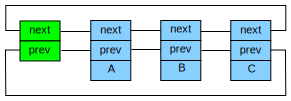
\includegraphics{defer/Linux_list}}
\caption{Linux Circular Linked List (\tco{list})}
\label{fig:defer:Linux Circular Linked List (list)}
\end{figure}

\begin{figure}[tb]
\centering
\resizebox{3in}{!}{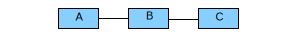
\includegraphics{defer/Linux_list_abbr}}
\caption{Linux Linked List Abbreviated}
\label{fig:defer:Linux Linked List Abbreviated}
\end{figure}

\co{rcu_assign_pointer()} 와 \co{rcu_dereference()} 가 이론상으로는 모든 상상할
수 있는 RCU 로 보호되는 데이터 구조를 만들 수 있지만, 실제로는 더 높은 단계의
것을 쓰는게 종종 낫습니다.
따라서, \co{rcu_assign_pointer()} 와 \co{rcu_dereference()} 는 리눅스의 리스트
조작 API 의 특수한 RCU 변종에 내포되어 있습니다.
리눅스는 네개의 양방향 링크드 리스트 변종을 갖는데, 순환형 \co{struct
list_head} 와 선형 \co{struct hlist_head}/\co{struct hlist_node}, \co{struct
hlist_nulls_head}/\co{struct hlist_nulls_node}, 그리고 \co{struct
hlist_bl_head}/\co{struct hlist_bl_node} 쌍들입니다.
앞의 것은
Figure~\ref{fig:defer:Linux Circular Linked List (list)} 에 보여져 있는 형태를
띄는데, (가장 왼쪽의) 녹색 상자가 리스트 헤더를 표현하며 (오른쪽 세개의) 파란
상자들은 이 리스트의 원소들을 표현합니다.
이 표기법은 다루기 성가시며 따라서 헤더가 아닌 (파랑) 원소들만 보이는
Figure~\ref{fig:defer:Linux Linked List Abbreviated} 에 보인 것처럼 간략화 할
겁니다.

\iffalse

Although \co{rcu_assign_pointer()} and
\co{rcu_dereference()} can in theory be used to construct any
conceivable RCU-protected data structure, in practice it is often better
to use higher-level constructs.
Therefore, the \co{rcu_assign_pointer()} and
\co{rcu_dereference()}
primitives have been embedded in special RCU variants of Linux's
list-manipulation API\@.
Linux has four variants of doubly linked list, the circular
\co{struct list_head} and the linear
\co{struct hlist_head}/\co{struct hlist_node},
\co{struct hlist_nulls_head}/\co{struct hlist_nulls_node}, and
\co{struct hlist_bl_head}/\co{struct hlist_bl_node}
pairs.
The former is laid out as shown in
Figure~\ref{fig:defer:Linux Circular Linked List (list)},
where the green (leftmost) boxes represent the list header and the blue
(rightmost three) boxes represent the elements in the list.
This notation is cumbersome, and will therefore be abbreviated as shown in
Figure~\ref{fig:defer:Linux Linked List Abbreviated},
which shows only the non-header (blue) elements.

\fi

\begin{figure}[tb]
\centering
\resizebox{3in}{!}{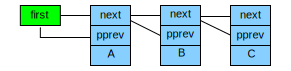
\includegraphics{defer/Linux_hlist}}
\caption{Linux Linear Linked List (\tco{hlist})}
\label{fig:defer:Linux Linear Linked List (hlist)}
\end{figure}

리눅스의 \co{hlist}\footnote{
	``h'' 는 해쉬테이블을 의미하는데, 리눅스의 양방향 포인터 순환형 링크드
	리스트에 비해 메모리 사용량을 절반으로 줄입니다.}
는 선형 리스트로, 이는
Figure~\ref{fig:defer:Linux Linear Linked List (hlist)}
에 보이듯헤더에  순환형 리스트에 필요한 두개의 포인터가 아니라 한개의 포인터만
필요합니다.
따라서, \co{hlist} 의 사용은 커다란 해쉬 테이블의 해쉬 버킷 배열을 위한 메모리
사용량을 절반으로 줄일 수 있습니다.
앞에서와 같이, 이 표기법은 다루기 귀찮으므로, \co{hlist} 구조는
Figure~\ref{fig:defer:Linux Linked List Abbreviated}
에 보인 것과 같은 \co{list_head} 스타일 리스트로 간략화 해 표기하겠습니다.

\iffalse

Linux's \co{hlist}\footnote{
	The ``h'' stands for hashtable, in which it reduces memory
	use by half compared to Linux's double-pointer circular
	linked list.}
is a linear list, which means that
it needs only one pointer for the header rather than the two
required for the circular list, as shown in
Figure~\ref{fig:defer:Linux Linear Linked List (hlist)}.
Thus, use of \co{hlist} can halve the memory consumption for the hash-bucket
arrays of large hash tables.
As before, this notation is cumbersome, so \co{hlist} structures will
be abbreviated in the same way \co{list_head}-style lists are, as shown in
Figure~\ref{fig:defer:Linux Linked List Abbreviated}.

\fi

\co{hlist_nulls} 라 이름지어진 리눅스의 \co{hlist} 의 한 변종은 여러 구별된
\co{NULL} 포인터들을 제공합니다만, 그것 외에는
Figure~\ref{fig:defer:Linux Linear Linked List (hlist)}
에 보인것과 같은 레이아웃을 갖습니다.
이 변종에서, 0 값의 낮은 위치 비트를 갖는 \co{->next} 포인터는 \co{NULL} 포인터
타입을 의미합니다.
이 타입의 리스트는 lockless 읽기 쓰레드들이 어떤 노드가 한 리스트에서 다른
리스트로 옮겨진 것을 파악할 수 있게 하기 위해 사용됩니다.
예를 들어, 해쉬 테이블의 각 버킷은 그것의 \co{NULL} 포인터를 마킹하기 위해 그
인덱스를 사용할 수도 있습니다.
읽기 쓰레드가 자신이 시작한 버킷의 인덱스와 맞지 않는 \co{NULL} 포인터를
마주치면, 이 읽기 쓰레드는 자신이 순회하고 있는 원소가 순회 사이에 다른
버킷으로 옮겨졌음을 알게 됩니다.
이 읽기 쓰레드는 리스트의 끝에 도달했는지 알기 위해 \co{is_a_nulls()} 함수
(\co{hlist_nulls} \co{NULL} 포인터를 받으면 true 를 리턴합니다) 를, \co{NULL}
포인터의 타입을 가져오기 위해 \co{get_nulls_value()} (이 함수는 인자의
\co{NULL} 포인터 식별자를 리턴합니다) 를 사용할 수 있습니다.
\co{get_nulls_value()} 가 예상치 않은 값을 리턴하면, 읽기 쓰레드는 올바른
행동을 취할 수 있는데, 예를 들면 시작부터 순회를 재시작 하는 것입니다.

\iffalse

A variant of Linux's \co{hlist}, named \co{hlist_nulls}, provides multiple
distinct \co{NULL} pointers, but otherwise uses the same layout as shown in
Figure~\ref{fig:defer:Linux Linear Linked List (hlist)}.
In this variant, a \co{->next} pointer having a zero low-order bit is
considered to be a pointer.
However, if the low-order bit is set to one, the upper bits identify
the type of \co{NULL} pointer.
This type of list is used to allow lockless readers to detect when a
node has been moved from one list to another.
For example, each bucket of a hash table might use its index to mark
its \co{NULL} pointer.
Should a reader encounter a \co{NULL} pointer not matching the index of
the bucket it started from, that reader knows that an element it was
traversing was moved to some other bucket during the traversal, taking
that reader with it.
The reader can use the \co{is_a_nulls()} function (which returns true
if passed an \co{hlist_nulls} \co{NULL} pointer) to determine when
it reaches the end of a list, and the \co{get_nulls_value()} function
(which returns its argument's \co{NULL}-pointer identifier) to fetch
the type of \co{NULL} pointer.
When \co{get_nulls_value()} returns an unexpected value, the reader
can take corrective action, for example, restarting its traversal from
the beginning.

\fi

\QuickQuiz{
	하지만 \co{hlist_nulls} 읽기 쓰레드가 다른 버킷으로 갔다가 다시
	돌아오면 어떻게 하죠?

	\iffalse

	But what if an \co{hlist_nulls} reader gets moved to some other
	bucket and then back again?

	\fi

}\QuickQuizAnswer{
	이를 제어하기 위한 한가지 방법은 항상 노드를 목적 버켓의 시작점으로
	옮겨서 읽기 쓰레드가 매치 되는 \co{NULL} 포인터를 갖는 리스트의 끝에
	닿았을 때에는 이 쓰레드가 이 리스트 전체를 탐색했음을 보장하는
	것입니다.

	물론, 해쉬 테이블에 버킷당 많은 원소가 있고 너무 많은 옮기기
	오퍼레이션이 존재한다면 읽기 쓰레드는 영영 리스트의 끝에 도달할 수 없을
	수도 있을 겁니다.
	평범한 경우에 이를 막는 한가지 방법은 해쉬 테이블을 잘 튜닝되어서 짧은
	리스트들만을 갖게 하는 것입니다.
	이 문제를 파악하고 처리하는 한가지 방법은 읽기 쓰레드가 어떤 많은 수의
	노드를 순회한 다음에는 탐색을 종료하고 update-side 락을 잡은 후 탐색을
	다시 하는 것이지만 이는 데드락을 초래할 수 있습니다.
	이 문제를 완전히 막는 또다른 방법은 읽기 쓰레드가 RCU read-side
	크리티컬 섹션 내에서 탐색을 하고, 이어지는 업데이트들 사이의 RCU grace
	period 하나를 기다리는 겁니다.
	중간의 위치는 어떤 적당한 $N$ 값을 가지고 매 $N$ 업데이트마다 RCU grace
	period 를 하나 기다릴 겁니다.

	\iffalse

	One way to handle this is to always move nodes to the beginning
	of the destination bucket, ensuring that when the reader reaches
	the end of the list having a matching \co{NULL} pointer, it will
	have searched the entire list.

	Of course, if there are too many move operations in a hash table
	with many elements per bucket, the reader might never reach the
	end of a list.
	One way of avoiding this in the common case is to keep hash
	tables well-tuned, thus with short lists.
	One way of detecting the problem and handling it is for the
	reader to terminate the search after traversing some large
	number of nodes, acquire the update-side lock, and redo the
	search, but this might introduce deadlocks.
	Another way of avoiding the problem entirely is for readers to
	search within RCU read-side critical sections, and to wait for
	an RCU grace period between successive updates.
	An intermediate position might wait for an RCU grace period
	every $N$ updates, for some suitable value of $N$.

	\fi

}\QuickQuizEnd

\co{hlist_nulls} 에 대한 더 많은 정보는 \path{rculist_nulls.rst} 파일 (오래된
커널에선 \path{rculist_nulls.txt}) 에서 제공되는 도움 될만한 예제 코드들과 함께
리눅스 커널의 소스 트리에서 얻을 수 있습니다.

리눅스의 \co{hlist} 의 또다른 변종은 비트 락킹을 결합하며, \co{hlist_bl} 이라
이름지어졌습니다.
이 변종은
Figure~\ref{fig:defer:Linux Linear Linked List (hlist)}
에 보인 것과 동일한 레이아웃을 사용하지만, 헤드 포인터의 (그림의 ``첫번째'')
낮은 위치 비트를 이 리스트를 잠그기 위해 사용됩니다.
이 방법 또한 메모리 사용량을 줄이는데, 이게 아니면 포인터 자체와 함께 별도의
스핀락이 저장되어야 하기 때문입니다.

\iffalse

More information on \co{hlist_nulls} is available in the Linux-kernel
source tree, with helpful example code provided in the
\path{rculist_nulls.rst} file (\path{rculist_nulls.txt} in older kernels).

Another variant of Linux's \co{hlist} incorporates bit-locking,
and is named \co{hlist_bl}.
This variant uses the same layout as shown in
Figure~\ref{fig:defer:Linux Linear Linked List (hlist)},
but reserves the low-order bit of the head pointer (``first'' in the
figure) to lock the list.
This approach also reduces memory usage, as it allows what would otherwise
be a separate spinlock to be stored with the pointer itself.

\fi

\begin{sidewaystable*}[htbp]
\rowcolors{1}{}{lightgray}
\renewcommand*{\arraystretch}{1.3}
\centering
\caption{RCU-Protected List APIs}
\label{tab:defer:RCU-Protected List APIs}
\footnotesize
\newlength{\cwa}\newlength{\cwb}\newlength{\cwc}\newlength{\cwd}
\IfNimbusAvail{
  \renewcommand{\ttdefault}{NimbusMonoN}
  \setlength{\cwa}{1.9in}\setlength{\cwb}{2.1in}
  \setlength{\cwc}{1.8in}\setlength{\cwd}{1.6in}
}{
  \setlength{\cwa}{1.95in}\setlength{\cwb}{2.15in}
  \setlength{\cwc}{1.9in}\setlength{\cwd}{1.7in}
}
\begin{tabular}{>{\raggedright\arraybackslash}p{\cwa}
    >{\raggedright\arraybackslash}p{\cwb}
    >{\raggedright\arraybackslash}p{\cwc}
    >{\raggedright\arraybackslash}p{\cwd}}
\toprule
\pmb{\tco{list}}: Circular doubly linked list &
    \pmb{\tco{hlist}}: Linear doubly linked list &
	\pmb{\tco{hlist_nulls}}: Linear doubly linked list with marked
	NULL pointer, with up to 31~bits of marking &
	    \pmb{\tco{hlist_bl}}: Linear doubly linked list with bit locking \\
\midrule
\multicolumn{4}{l}{{\bf Structures}} \\
\tco{struct list_head} &
    \tco{struct}{\tt ~}\tco{hlist_head} ~~~~~~~~~~~~~~
    \tco{struct}{\tt ~}\tco{hlist_node} &
	\tco{struct}{\tt ~}\tco{hlist_nulls_head}
	\tco{struct}{\tt ~}\tco{hlist_nulls_node} &
	    \tco{struct}{\tt ~}\tco{hlist_bl_head}
	    \tco{struct}{\tt ~}\tco{hlist_bl_node} \\
\multicolumn{4}{l}{{\bf Initialization}} \\
&
    \tco{INIT_LIST_HEAD_RCU()} &
	&
	    \\
\multicolumn{4}{l}{{\bf Full traversal}} \\
\tco{list_for_each_entry_rcu()}
\tco{list_for_each_entry_lockless()} &
    \tco{hlist_for_each_entry_rcu()}
    \tco{hlist_for_each_entry_rcu_bh()}
    \tco{hlist_for_each_entry_rcu_notrace()} &
	\tco{hlist_nulls_for_each_entry_rcu()}
	\tco{hlist_nulls_for_each_entry_safe()} &
	    \tco{hlist_bl_for_each_entry_rcu()} \\
\multicolumn{4}{l}{{\bf Resume traversal}} \\
\tco{list_for_each_entry_continue_rcu()}
\tco{list_for_each_entry_from_rcu()} &
    \tco{hlist_for_each_entry_continue_rcu()}
    \tco{hlist_for_each_entry_continue_rcu_bh()}
    \tco{hlist_for_each_entry_from_rcu()} &
	&
	    \\
\multicolumn{4}{l}{{\bf Stepwise traversal}} \\
\tco{list_entry_rcu()}
\tco{list_entry_lockless()}
\tco{list_first_or_null_rcu()}
\tco{list_next_rcu()}
\tco{list_next_or_null_rcu()} &
    \multicolumn{1}{p{1.2in}}{\tco{hlist_first_rcu()}
			      \tco{hlist_next_rcu()}
			      \tco{hlist_pprev_rcu()}} &
	\tco{hlist_nulls_first_rcu()}
	\tco{hlist_nulls_next_rcu()} &
	    \tco{hlist_bl_first_rcu()} \\
\multicolumn{4}{l}{{\bf Add}} \\
\multicolumn{1}{p{1.2in}}{\tco{list_add_rcu()}
			  \tco{list_add_tail_rcu()}} &
    \tco{hlist_add_before_rcu()}
    \tco{hlist_add_behind_rcu()}
    \tco{hlist_add_head_rcu()}
    \tco{hlist_add_tail_rcu()} &
	\tco{hlist_nulls_add_head_rcu()} &
	    \tco{hlist_bl_add_head_rcu()}
	    \tco{hlist_bl_set_first_rcu()} \\
\multicolumn{4}{l}{{\bf Delete}} \\
\tco{list_del_rcu()} &
    \multicolumn{1}{p{1.2in}}{\tco{hlist_del_rcu()}
			      \tco{hlist_del_init_rcu()}} &
	\tco{hlist_nulls_del_rcu()}
	\tco{hlist_nulls_del_init_rcu()} &
	    \tco{hlist_bl_del_rcu()}
	    \tco{hlist_bl_del_init_rcu()} \\
\multicolumn{4}{l}{{\bf Replace}} \\
\tco{list_replace_rcu()} &
    \tco{hlist_replace_rcu()} &
	&
	    \\
\multicolumn{4}{l}{{\bf Splice}} \\
\tco{list_splice_init_rcu()} &
    \tco{list_splice_tail_init_rcu()} &
	&
	    \\
\bottomrule
\end{tabular}
\end{sidewaystable*}

The API members for these linked-list variants are summarized in
Table~\ref{tab:defer:RCU-Protected List APIs}.
More information is available in the \path{Documentation/RCU}
directory of the Linux-kernel source tree and at
Linux Weekly News~\cite{PaulEMcKenney2019RCUAPI}.

However, the remainder of this section expands on the use of
\co{list_replace_rcu()}, given that this API member gave RCU its name.
This API member is used to carry out more complex updates in which an
element in the middle of the list having multiple fields is atomically
updated, so that a given reader sees either the old set of values or
the new set of values, but not a mixture of the two sets.
For example, each node of a linked list might have integer fields
\co{->a}, \co{->b}, and~\co{->c}, and it might be necessary to update
a given node's fields from 5, 6, and~7 to 5, 2, and~3, respectively.

The code implementing this atomic update is straightforward:

\begin{fcvlabel}[ln:defer:Canonical RCU Replacement Example (2nd)]
\begin{VerbatimN}[samepage=true,commandchars=\\\[\],firstnumber=15]
q = kmalloc(sizeof(*p), GFP_KERNEL);	\lnlbl[kmalloc]
*q = *p;				\lnlbl[copy]
q->b = 2;				\lnlbl[update1]
q->c = 3;				\lnlbl[update2]
list_replace_rcu(&p->list, &q->list);	\lnlbl[replace]
synchronize_rcu();			\lnlbl[sync_rcu]
kfree(p);				\lnlbl[kfree]
\end{VerbatimN}
\end{fcvlabel}

\begin{figure}[tbp]
\centering
\resizebox{2.7in}{!}{\includegraphics{defer/RCUReplacement}}
\caption{RCU Replacement in Linked List}
\label{fig:defer:RCU Replacement in Linked List}
\end{figure}

The following discussion walks through this code, using
Figure~\ref{fig:defer:RCU Replacement in Linked List} to illustrate
the state changes.
The triples in each element represent the values of fields \co{->a},
\co{->b}, and \co{->c}, respectively.
The red-shaded elements might be referenced by readers,
and because readers do not synchronize directly with updaters,
readers might run concurrently with this entire replacement process.
Please note that backwards pointers and the link from the tail to the
head are omitted for clarity.

The initial state of the list, including the pointer \co{p},
is the same as for the deletion example, as shown on the
first row of the figure.

The following text describes how to replace the \co{5,6,7} element
with \co{5,2,3} in such a way that any given reader sees one of these
two values.

\begin{fcvref}[ln:defer:Canonical RCU Replacement Example (2nd)]
Line~\lnref{kmalloc} allocates a replacement element,
resulting in the state as shown in the second row of
Figure~\ref{fig:defer:RCU Replacement in Linked List}.
At this point, no reader can hold a reference to the newly allocated
element (as indicated by its green shading), and it is uninitialized
(as indicated by the question marks).

Line~\lnref{copy} copies the old element to the new one, resulting in the
state as shown in the third row of
Figure~\ref{fig:defer:RCU Replacement in Linked List}.
The newly allocated element still cannot be referenced by readers, but
it is now initialized.

Line~\lnref{update1} updates \co{q->b} to the value ``2'', and
line~\lnref{update2} updates \co{q->c} to the value ``3'',
as shown on the fourth row of
Figure~\ref{fig:defer:RCU Replacement in Linked List}.
Note that the newly allocated structure is still inaccessible to readers.

Now, line~\lnref{replace} does the replacement, so that the new element is
finally visible to readers, and hence is shaded red, as shown on
the fifth row of
Figure~\ref{fig:defer:RCU Replacement in Linked List}.
At this point, as shown below, we have two versions of the list.
Pre-existing readers might see the \co{5,6,7} element (which is
therefore now shaded yellow), but
new readers will instead see the \co{5,2,3} element.
But any given reader is guaranteed to see one set of values or the
other, not a mixture of the two.

After the \co{synchronize_rcu()} on line~\lnref{sync_rcu} returns,
a grace period will have elapsed, and so all reads that started before the
\co{list_replace_rcu()} will have completed.
In particular, any readers that might have been holding references
to the \co{5,6,7} element are guaranteed to have exited
their RCU read-side critical sections, and are thus prohibited from
continuing to hold a reference.
Therefore, there can no longer be any readers holding references
to the old element, as indicated its green shading in the sixth row of
Figure~\ref{fig:defer:RCU Replacement in Linked List}.
As far as the readers are concerned, we are back to having a single version
of the list, but with the new element in place of the old.

After the \co{kfree()} on line~\lnref{kfree} completes, the list will
appear as shown on the final row of
Figure~\ref{fig:defer:RCU Replacement in Linked List}.
\end{fcvref}

Despite the fact that RCU was named after the replacement case,
the vast majority of RCU usage within the Linux kernel relies on
the simple independent insertion and deletion, as was shown in
Figure~\ref{fig:defer:Multiple RCU Data-Structure Versions} in
Section~\ref{sec:defer:Maintain Multiple Versions of Recently Updated Objects}.

The next section looks at APIs that assist developers in debugging
their code that makes use of RCU\@.

\subsubsection{RCU Has Diagnostic APIs}
\label{sec:defer:RCU Has Diagnostic APIs}

\begin{table}[tb]
\renewcommand*{\arraystretch}{1.15}
\footnotesize
\centering
\begin{tabular}{ll}
\toprule
Category &
	Primitives \\
\midrule
Mark RCU pointer &
	\tco{__rcu} \\
\midrule
Debug-object support &
	\tco{init_rcu_head()} \\
&	\tco{destroy_rcu_head()} \\
&	\tco{init_rcu_head_on_stack()} \\
&	\tco{destroy_rcu_head_on_stack()} \\
\midrule
Stall-warning control &
	\tco{rcu_cpu_stall_reset()} \\
\midrule
Callback checking &
	\tco{rcu_head_init()} \\
&	\tco{rcu_head_after_call_rcu()} \\
\midrule
lockdep support &
	\tco{rcu_read_lock_held()} \\
&	\tco{rcu_read_lock_bh_held()} \\
&	\tco{rcu_read_lock_sched_held()} \\
&	\tco{srcu_read_lock_held()} \\
&	\tco{rcu_is_watching()} \\
&	\tco{RCU_LOCKDEP_WARN()} \\
&	\tco{RCU_NONIDLE()} \\
&	\tco{rcu_sleep_check()} \\
\bottomrule
\end{tabular}
\caption{RCU Diagnostic APIs}
\label{tab:defer:RCU Diagnostic APIs}
\end{table}

Table~\ref{tab:defer:RCU Diagnostic APIs}
shows RCU's diagnostic APIs.

The \co{__rcu} marks an RCU-protected pointer, for example,
\qtco{struct foo __rcu *p;}.
Pointers that might be passed to \co{rcu_dereference()} can be marked,
but pointers holding values returned from \co{rcu_dereference()}
should not be.
Providing these markings on variables, structure fields, function
parameters, and return values allow the Linux kernel's \co{sparse}
tool to detect situtations where RCU-protected pointers are
incorrectly accessed using plain C-language loads and stores.

Debug-object support is automatic for any \co{rcu_head} structures
that are part of a structure obtained from the Linux kernel's
memory allocators, but those building their own special-purpose
memory allocators can use \co{init_rcu_head()} and \co{destroy_rcu_head()}
at allocation and free time, respectively.
Those using \co{rcu_head} structures allocated on the function-call
stack (it happens!) may use \co{init_rcu_head_on_stack()}
before first use and \co{destroy_rcu_head_on_stack()} after last use,
but before returning from the function.
Debug-object support allows detection of bugs involving passing the
same \co{rcu_head} structure to \co{call_rcu()} and friends in
quick succession, which is the \co{call_rcu()} counterpart to the
infamous double-free class of memory-allocation bugs.

Stall-warning control is provided by \co{rcu_cpu_stall_reset()}, which
allows the caller to suppress RCU CPU stall warnings for the remainder
of the current grace period.
RCU CPU stall warnings help pinpoint situations where an RCU read-side
critical section runs for an excessive length of time, and it is useful
for things like kernel debuggers to be able to suppress them, for example,
when encountering a breakpoint.

Callback checking is provided by \co{rcu_head_init()} and
\co{rcu_head_after_call_rcu()}.
The former is invoked on an \co{rcu_head} structure before it is passed
to \co{call_rcu()}, and then \co{rcu_head_after_call_rcu()} will
check to see if the callback is has been invoked with the specified
function.

Support for lockdep~\cite{JonathanCorbet2006lockdep} includes
\co{rcu_read_lock_held()},
\co{rcu_read_lock_bh_held()},
\co{rcu_read_lock_sched_held()}, and
\co{srcu_read_lock_held()},
each of which returns \co{true} if invoked within the corresponding
type of RCU read-side critical section.

\QuickQuiz{
	Why isn't there a \co{rcu_read_lock_tasks_held()} for Tasks RCU?
}\QuickQuizAnswer{
	Because Tasks RCU does not have read-side markers.
	Instead, Tasks RCU read-side critical sections are
	bounded by voluntary context switches.
}\QuickQuizEnd

Because \co{rcu_read_lock()} cannot be used from the idle loop,
and because energy-efficiency concerns have caused the idle loop
to become quite ornate, \co{rcu_is_watching()} returns true if
invoked in a context where use of \co{rcu_read_lock()} is legal.
Note again that \co{srcu_read_lock()} may be used from idle and
even offline CPUs, which means that \co{rcu_is_watching()} does not
apply to SRCU\@.

\co{RCU_LOCKDEP_WARN()} emits a warning if lockdep is enabled and if
its argument evaluated to \co{true}.
For example, \co{RCU_LOCKDEP_WARN(!rcu_read_lock_held())} would emit a
warning if invoked outside of an RCU read-side critical section.

\co{RCU_NONIDLE()} may be used to force RCU to watch when executing
the statement that is passed in as the sole argument.
For example, \co{RCU_NONIDLE(WARN_ON(!rcu_is_watching()))}
would never emit a warning.
However, changes in the 2020--2021 timeframe extend RCU's reach deeper
into the idle loop, which should greatly reduce or even eliminate the
need for \co{RCU_NONIDLE()}.

Finally,  \co{rcu_sleep_check()} emits a warning if invoked within
an RCU, RCU-bh, or RCU-sched read-side critical section.

\subsubsection{Where Can RCU's APIs Be Used?}
\label{sec:defer:Where Can RCU's APIs Be Used?}

\begin{figure}[tb]
\centering
\resizebox{3in}{!}{\includegraphics{defer/RCUenvAPI}}
\caption{RCU API Usage Constraints}
\label{fig:defer:RCU API Usage Constraints}
\end{figure}

Figure~\ref{fig:defer:RCU API Usage Constraints}
shows which APIs may be used in which in-kernel environments.
The RCU read-side primitives may be used in any environment, including NMI,
the RCU mutation and asynchronous grace-period primitives may be used in any
environment other than NMI, and, finally, the RCU synchronous grace-period
primitives may be used only in process context.
The RCU list-traversal primitives include \co{list_for_each_entry_rcu()},
\co{hlist_for_each_entry_rcu()}, etc.
Similarly, the RCU list-mutation primitives include
\co{list_add_rcu()}, \co{hlist_del_rcu()}, etc.

Note that primitives from other families of RCU may be substituted,
for example, \co{srcu_read_lock()} may be used in any context
in which \co{rcu_read_lock()} may be used.

\subsubsection{So, What \emph{is} RCU Really?}
\label{sec:defer:So, What is RCU Really?}

At its core, RCU is nothing more nor less than an API that supports
publication and subscription for insertions, waiting for all RCU readers
to complete, and maintenance of multiple versions.
That said, it is possible to build higher-level constructs
on top of RCU, including the reader-writer-locking, reference-counting,
and existence-guarantee constructs listed in
Section~\ref{sec:defer:RCU Usage}.
Furthermore, I have no doubt that the Linux community will continue to
find interesting new uses for RCU,
just as they do for any of a number of synchronization
primitives throughout the kernel.

Of course, a more-complete view of RCU would also include
all of the things you can do with these APIs.

However, for many people, a complete view of RCU must include sample
RCU implementations.
Appendix~\ref{chp:app:``Toy'' RCU Implementations} therefore presents a series
of ``toy'' RCU implementations of increasing complexity and capability,
though others might prefer the classic
``User-Level Implementations of Read-Copy
Update''~\cite{MathieuDesnoyers2012URCU}.
For everyone else, the next section gives an overview of some RCU use cases.
